%!TEX root = ../thesis.tex
%*******************************************************************************
%****************************** Third Chapter **********************************
%*******************************************************************************
\chapter{Digitalización de secuencias lineales de proteínas aplicadas al reconocimiento de patrones y modelos predictivos \label{cap3}}

% **************************** Define Graphics Path **************************
\ifpdf
    \graphicspath{{Chapter3/Figs/Raster/}{Chapter3/Figs/PDF/}{Chapter3/Figs/}}
\else
    \graphicspath{{Chapter3/Figs/Vector/}{Chapter3/Figs/}}
\fi

Desarrollar modelos predictivos basados en algoritmos de aprendizaje supervisado, o, la identificación de patrones aplicando técnicas de clustering, son tareas muy relevantes a la hora de trabajar con secuencias de proteínas, ya sea para identificar grupos con características comunes o entrenar modelos predictivos de respuestas de interés. En ambos casos, se requiere el uso de conjuntos de datos altamente informativos y con características numéricas para poder utilizar los métodos implementados en las librerías actuales \cite{pedregosa2011scikit}.

Diferentes metodologías se han implementado, para manipular las variables categóricas en set de datos y lograr su codificación numérica. Enfoques basados en adición de columnas según las categorías o simple transformación empleando representaciones en conjuntos naturales, suelen ser utilizados. No obstante, generan bastante discusión sobre las nuevas representaciones. y a su vez, el hecho de aumentar el número de columnas, conlleva a incrementar las dimensiones del conjunto de datos, provocando efectos en los desempeños de los algoritmos \cite{pedregosa2011scikit}. 

Particularmente, en secuencias de proteínas, se han utilizado las frecuencias de incidencia de los residuos para codificarlos, la cual, pese a su simplicidad, ha resultado ser efectiva en diferentes casos de uso \cite{ozbudak2014protein}. No obstante, este tipo de codificación, no permite explorar el ambiente bajo el cual se encuentran los residuos y tampoco considera el efecto de propiedades fisicoquímicas ni termodinámicas.

En diferentes estudios, los residuos se describen a partir de sus propiedades fisicoquímicas y adicional a ello, se emplea información que permite describir el ambiente del residuo a caracterizar, empleando binarizaciones para describir los residuos cercanos, ya sea por medio del uso de un rango espacial, utilizando modelos o estructuras tridimensionales en donde se representan las coordenadas espaciales de los residuos, o empleando un rango lineal en secuencias lineales de proteínas \cite{capriotti2005mutant2, capriotti2008three}.

Un enfoque basado en las propiedades fisicoquímicas en combinación con la aplicación de transformaciones de Fourier, ha permitido demostrar que ciertos residuos permiten entregar las características asociadas a la propiedad en estudio, además, facilita comprender el aporte del ambiente sobre estos y representa una forma de estudio novedosa para el uso de información de secuencias lineales. Siendo una metodología ampliamente utilizada para identificar residuos que aporten a la propiedad, por medio de la representación de señales asociadas al espacio de frecuencias \cite{veljkovic1985possible, cosic2016analysis, cadet2018application}.

A pesar de ser una metodología interesante a la hora de estudiar secuencias lineales, exhiben problemas notorios sobre la selección de las propiedades relevantes a analizar, ya que, existe un número considerablemente alto de propiedades posibles a utilizar, descritas principalmente en las base de datos AAIndex \cite{Kawashima2000}, y es factible que diferentes familias de proteínas exhiban comportamientos notoriamente no similares y diverjan en cuanto a las propiedades que puedan ser representativas, inclusive, a la hora de estudiar mutaciones en una misma proteína puede que no sólo una propiedad permita su caracterización, si no, que un conjunto pequeño de éstas \cite{cadet2018application}.

En el presente capítulo, se exponen en detalle, diferentes formas de representar secuencias lineales de proteínas, seguido a su vez del planteamiento del uso de transformadas de Fourier para la digitalización de propiedades fisicoquímicas y cómo es posible utilizar éstas para la identificación de patrones en secuencias lineales o el desarrollo de modelos de clasificación/regresión y la exposición de casos de uso en diferentes proteínas de interés. 

\section{Metodologías asociadas a la codificación de variables categóricas}

Diferentes metodologías existen para poder codificar variables categóricas, a su vez, para set de datos de proteínas con secuencias lineales, es factible utilizar sus propiedades fisicoquímicas o frecuencias de residuos. Las principales metodologías usadas a la fecha se expone a continuación.

\subsection{One Hot encoder}

One Hot encoder, es una de las técnicas más utilizadas a la hora de codificar variables categóricas y se basa principalmente en la adición de columnas con respecto a las categorías existentes en un conjunto de datos \cite{brownlee2017one}.

Dado el vector  $x$ de tamaño $n$ con $m$ categorías, por definición, One Hot encoder agrega al conjunto de datos $m$ columnas, tal que, por cada categoría se adiciona una nueva columna al set de datos. Las nuevas columnas se completan con una binarización de los elementos, indicando si el elemento $x_{i}$ posee la categoría $m_{j}$ con un valor 1 y en caso contrario 0. Es posible expresar esto como se expone a continuación.

Sea $x$ vector de $m$ categorías de dimensiones
$n \times 1$ representado por
\[ x = \left( \begin{array}{ccc}
x_{0}\\
x_{1}\\
\vdots\\
x_{n-1} \end{array} \right)\] 
Su codificación mediante One Hot Encoder corresponde al vector x'(x)
\[ x'(x) = \left( \begin{array}{ccccc}
1 & 0 & 0 & \cdots & 0 \\
0 & 1 & 0 & \cdots & 0 \\
\vdots\\
0 & 0 & 0 & \cdots & 1 \end{array} \right) \] 

Esta metodología, si bien es altamente usada, implica que, a medida que aumentan la cantidad de categorías incrementan el número de columnas a agregar en el set de datos, es decir, si se tienen $m$ categorías se adicionan $m$ columnas. Esto último, puede provocar que los set de datos se afecten por problemas relacionados con la \textit{maldición de dimensionalidad} \footnote{Ver sección \ref{problemas}}, ya que, a medida que aumentan los descriptores, aumenta la probabilidad de que estos no sean informativos, provocando una adición de información innecesaria y que perjudicaría el rendimiento de los algoritmos de aprendizajes supervisado y no supervisado.

\subsection{Ordinal encoder}

Ordinal encoder, es una simplicación de One Hot encoder, ya que, simplemente codifica las categorías con números en el conjunto $[0, m-1]$. Es decir, sea el vector $x$ de tamaño $n$ con $m$ categorías y sea $M$ el espacio de las posibles categorías con $M = [m_{1}, \cdots, m_{m}]$, y cuya codificación implica el vector $M' = [0, \cdots, m-1]$. $\forall $ elemento que $\in$ a $x$ se obtiene su codificación a partir del elemento $M'(M(m_{i}))$ que corresponde a la codificación de la categoría en el espacio $M$ \cite{pedregosa2011scikit}.

Es posible cuestionar esta metodología con respecto al orden en que trata las categorías, la representación de la información y el mantenimiento del significado de la data. Razón por la cual, se usa sólo en los casos en que la adición de múltiples descriptores empleando One Hot Encoder sea perjudicial a la hora de implementar modelos de clasificación o regresión, e inclusive, en la búsqueda de patrones.

\subsection{Frecuencias de residuos}

Una secuencia lineal de proteína, corresponde a un vector $v$ de tamaño $n$ donde cada elemento corresponde a un residuo que pertenece a la secuencia. El uso de esta información para alimentar modelos de clasificación o regresión conlleva la codificación de sus elementos. Sin embargo, a la hora de utilizar las codificaciones basadas en One Hot Encoder, el conjunto de datos no queda estándar en cuanto a sus dimensiones, ya que, el largo de las secuencias puede variar y a su vez, el número de columnas a agregar corresponde a $n \times 20$ dado a que son $n$ residuos y el espacio muestral $M$ es de tamaño 20 lo que genera un aumento considerable en la cantidad de dimensiones.

Con el fin de poder representar las secuencias lineales de proteínas, se idearon metodologías que consideran la frecuencia de aparición de los residuos en la secuencia, de tal manera, de poder codificarla en un vector de tamaño 20, donde cada elemento representa el número de incidencias del residuo dividido por el largo del vector. Así, cada elemento se encuentra en un rango $[0,1]$ donde 0 indica no incidencia del residuo y 1, incidencia total \cite{ozbudak2014protein}.

Expresado de forma matemática, sea $s$ una secuencia lineal de proteínas con $r$ residuos, su codificación se basa en la frecuencia de aparición del residuo en $s$, tal que, sea $R$ el espacio de los posibles residuos $r$ en $s$, se estima para cada $r_{j} \in\ R$ su frecuencia:

\begin{equation}
	frec(r_{j}) = \dfrac{cont(r_{j})\ if\  (r_{i}==r_{j})}{n}
\end{equation}

Finalmente, se tiene que cada residuo $r_{i}$ se representa en su valor de frecuencia $frec(r_{i})$, generando un set de datos de tamaños $s \times 20$ con $s$ secuencias representadas por un vector de tamaño 20.

Esta es una de las representaciones más utilizadas y más simples a la hora de codificar secuencias lineales de proteínas. Sin embargo, presenta diferentes problemas tales como:

\begin{itemize}
	
	\item Si los residuos se encuentran en proporciones similares, se generarán conjuntos de datos con atributos no informativos, ya que, disminuirá la varianza existente para dicho atributo, provocando una redundancia de datos.
	
	\item No considera información sobre los residuos asociados a propiedades fisicoquímicas, esto complica el hecho de representar un set de datos de secuencias o mutaciones, ya que no representa la realidad y sólo expone el comportamiento de las frecuencias de residuos, favoreciendo a aquellos con una mayor incidencia en sus elementos.
	
	\item La codificación por frecuencias es utilizada como un primer acercamiento a la representación del problema y principalmente perjudica a los modelos ya que puede generar atributos no informativos, como lo son los residuos sin incidencia, esto conlleva a modelos sobre ajustados y a creación de set de datos no informativos.
	
	\item No evalúa elementos relevantes a la caracterización de residuos claves, ambiente bajo el cual ocurren mutaciones o componentes adicionales que facilitarían una mayor comprensión del problema, ya que, sólo conocer las incidencias, proporciona un conocimiento sobre la moda y cuáles son los residuos más relevantes. No obstante, sólo permite inferir características, relacionadas a estos.
\end{itemize}

El uso de las frecuencias de residuos, es una de las primeras aproximaciones a la codificación de secuencias lineales de proteínas. No obstante, en todos los casos donde han sido utilizadas, se agrega información adicional, que permite comprender diferentes comportamientos y evalúa ciertas propiedades del entorno, razones por las cuales, se recomiendan utilizarlas en conjunto con otros descriptores. 

\subsection{Uso de propiedades fisicoquímicas}

El uso de propiedades fisicoquímicas para describir un residuo, es ampliamente empleado en la generación de descriptores para conjuntos de datos en ingeniería de proteínas \cite{capriotti2005mutant2, capriotti2008three}. Diversos enfoques y modelos han sido construidos o entrenados, contemplando información asociada a componentes termodinámicos del residuo, en particular, a la hora de describir residuos para evaluar cambios en la energía libre, relacionados a efectos en la estabilidad de una proteína \cite{ancien2018prediction, broom2017computational, 1gzp030}.

Se han reportado cerca de 570 propiedades fisicoquímicas que pueden ser utilizadas para describir un residuo en una secuencia lineal de proteínas, almanceadas en la base de datos AAIndex \cite{Kawashima2000}. A su vez, es posible caracterizar estos residuos empleando un conjunto de propiedades estructurales, termodinámicas e inclusive filogenéticas. Es decir, diferentes puntos de vista que permitan describir los residuos pertenecientes a una secuencia. Sin embargo, el hecho de seleccionar qué descriptores son relevantes y cuáles no, radica en un problema de evaluación de características, el cual es común, en el área de la minería de datos. 

Dado al gran conjunto de propiedades existentes y a la diversidad de descriptores que pueden ser utilizados para un conjunto de secuencias lineales de proteínas, es necesaria una selección correcta de las características, las cuales permitan formar set de datos informativos y con una correlación mínima entre sus elementos. 

Contemplando esta problemática, técnicas de reducción de dimensionalidad o análisis de características son las más utilizadas a la hora de seleccionar los descriptores más informativos para un conjunto de datos. No obstante, en ocasiones, el conocimiento sobre el problema es un factor relevante a considerar. 

Dada la relevancia de la selección de descriptores correctos para poder caracterizar y codificar secuencias lineales a partir de propiedades, se describen a continuación, algunas técnicas de reducción de dimensionalidad y análisis de características que pueden ser empleadas para dar solución a esta problemática.

\subsubsection{Técnicas de reducción de dimensionalidad}

Diferentes técnicas para el análisis de características y reducción de dimensionalidad han sido implementadas en el campo de minería de datos, con el fin de poder permitir la selección de descriptores informativos y sin contemplar conjuntos de datos altamente dimensionales. Dentro de las principales destacan: Análisis de correlación, mutual information, evaluaciones de características con respecto al entrenamiento de modelos empleando Random Forest, Análisis de componentes principales (PCA) y sus variantes como métodos lineales y reducción de dimensionalidad empleando métodos no lineales. 

\subsubsection{Análisis de correlación}

La correlación entre elementos, es posible definirla como una relación estadística entre dos variables aleatorias, asociado principalmente, a relacionales lineales entre ellas \cite{cohen2014applied}. Existen diferentes coeficientes de correlación, dentro de los cuales, el más conocido es Pearson. No obstante, se encuentran además: Spearman rank, kendall $\tau$. La formulación matemática de estos, fue expuesta en la sección \ref{desempeno}, en el apartado de análisis de desempeño de modelos de regresión.

De manera general, la correlación se relaciona con la covarianza entre las variables aleatorias \cite{cohen2014applied}, esto es: Sean $X$ e $Y$ variables aleatorias, el coeficiente de correlación $\rho$ entre ellas se define como:

\begin{equation}
	\rho (X,Y) = corr(X,Y) = \dfrac{cov(X,Y)}{\sigma_{Y}\sigma_{Y}} = \dfrac{E[(X - \mu_{X})(Y - \mu_{Y})]}{\sigma_{Y}\sigma_{Y}}
\end{equation}

$\rho \in [-1, 1]$ de tal forma que -1 indica una correlación inversa entre los elementos y 1 una relación positiva. En efectos prácticos, ambos valores denotan una dependencia entre los elementos, por lo que no son informativos y es posible eliminar uno de ellos, dada la redundancia de información. Valores cercanos a 0, indican que las variables no se encuentran correlacionadas.

Estos estudios se realizan para todas las variables en un conjunto de datos, expresándose en matrices de correlación, las cuales, pueden ser visualizadas mediante Heat Map en donde se expone la dependencia entre los atributos. Siendo una de las técnicas más utilizadas para la reducción de dimensionalidad, debido a su simpleza y a las ventajas que posee con respecto a la información que entrega sobre los atributos.

\subsubsection{Mutual information}

Es una medida de dependencia mutua entre dos variables aleatorias, permitiendo cuantificar la cantidad de información obtenida alrededor de una variable aleatoria vista desde otra. Representa un concepto más general que el análisis de correlación y se basa en la comparación de la similitud entre las distribuciones del conjunto de las variables independientes, con respecto al producto de éstas \cite{peng2005feature}.

Sean dos variables aleatorias $X$ e $Y$ con valores en el espacio $X \times Y$ y sea el conjunto $P_{(X,Y)}$ y las distribuciones marginales son $P_X$ y $P_Y$, respectivamente. El mutual information score para las variables $X$ e $Y$ es:

\begin{equation}
	I(X,Y) = D_{KL}(P_{(X,Y)} || P_X \otimes P_Y)
\end{equation}

Esto puede variar con respecto al tipo de variable a utilizar. En el caso de que pertenezcan a una distribución discreta el $I(X,Y)$ corresponde a:

\begin{equation}
	I(X,Y) = \sum_{y_{i} \in Y} \sum_{x \in X} P_{(x,y)} (x,y) \log (\dfrac{P_{(x,y)}(x,y)}{P_{x}(x)P_{y}(y)})
\end{equation}

Mientras que para el caso de variables con distribución continua se tiene:

\begin{equation}
	I(X,Y) = \int_{y} \int_{x} P_{(x,y)} (x,y) \log (\dfrac{P_{(x,y)}(x,y)}{P_{x}(x)P_{y}(y)})
\end{equation}

Como interpretación, se tiene que presenta un rango de valores no negativos, donde un valor 0 indica que no existe información mutua entre ambas características y a mayor valor más relación existe entre ambos elementos.

\subsubsection{Análisis espaciales de características}

En la sección \ref{rf}, se describió Random Forest como un algoritmo de aprendizaje supervisado, que permite entrenar modelos utilizando árboles de decisión para manipular las características, generando $n$ iteraciones, en donde se construyen $n$ árboles, con diferentes atributos y ejemplos. Esto, permite estabilizar las medidas de desempeño y generar modelos robustos y con probabilidades menores de sobreajuste.

Sin embargo, este método puede ser utilizado con el fin de evaluar las características, ya sea en torno a cuáles son las frecuencias con las que permite dividir de manera inicial el conjunto de datos o cuáles son las que permiten generar la clasificación o la asignación a un intervalo en términos de regresión \cite{saeys2008robust}. 

A partir de lo anterior, la profundidad de una característica utilizada como nodo de decisión en un árbol puede usarse para evaluar la importancia relativa de esa característica con respecto a la predictibilidad de la variable objetivo. Las características utilizadas en la parte superior del árbol contribuyen a la decisión de predicción final de una fracción mayor de las muestras de entrada. La fracción esperada de las muestras a las que contribuyen puede, por lo tanto, usarse como una estimación de la importancia relativa de las características \cite{granitto2006recursive}. 

La fracción de muestras a las que contribuye una característica se combina con la disminución de la impureza al dividirlas para crear una estimación normalizada del poder predictivo de esa característica \cite{saeys2008robust}.

\subsubsection{Métodos de reducción de dimensionalidad lineales}

Reducción de dimensionalidad, como su nombre lo sugiere, implica remover características o atributos del set de datos, con el objetivo de disminuir el número de dimensiones del conjunto de elementos. Esto permite descartar los atributos menos informativos o con menor relevancia, ya sea en términos de aporte a la varianza o relaciones con el resto de descriptores \cite{hinton2006reducing}.

Dentro de las principales técnicas de reducción lineales, se encuentran el Análisis de componentes principales (PCA) y sus variantes, tales como: Incremental PCA \cite{jolliffe2011principal}, Non-negative matrix factorization (NMF), Linear discriminant analysis (LDA), dentro de los principales, siendo el más utilizado PCA, razón por la cual se exponen de manera breve sus características y definiciones a continuación. 

Análisis de Componentes Principales (PCA, por sus iniciales en inglés), es una técnica estadística que permite la conversión de un conjunto de variables posiblemente correlacionadas a un conjunto de variables no correlacionadas linealmente. Estos elementos se denominan componentes principales. Su principal característica es que son ordenados de mayor a menor, según la varianza que entregan a los datos \cite{jolliffe2011principal}.

Intuitivamente, es posible pensar el PCA como un elipsoide n-dimensional de datos, donde cada eje del elipsoide representa un componente principal. Esto implica, que si algún eje del elipsoide es pequeño, la varianza correspondiente a lo largo de éste también lo es, por lo que omitir dicho eje no implica una pérdida importante de información, lo cual es denotado como la reducción de la dimensionalidad en base a los aportes a las varianzas que denotan cada componente \cite{wold1987principal}.

\paragraph{Definición\\\\}

Matemáticamente, es posible definir PCA como una transformación lineal ortogonal de los datos a un nuevo sistema de coordenadas, tal que, la mayor varianza por alguna proyección de los datos pasa a situarse en la primera coordenada (llamado el primer componente principal), la segunda mayor varianza en la segunda coordenada, y así sucesivamente.

Se considera un conjunto de datos, $X$, con una media empírica 0, donde cada una de las filas  representan ejemplos y las columnas características o atributos $p$.

La transformación está definida por un set de vectores de dimensión $p$ que poseen pesos denotados por $ w_{(k)} = (w_{1},...,w_{p})_{(k)}$, los cuales para cada vector $x_{i}$ en $X$ se operan para dar un vector con los componentes principales $ t_{(i)} = (t_{1},...,t_{k})_{(i)}$ el cual viene dado por $ t_{k(i)} = x_{i}  w_{k}$

De tal manera que las variables individuales de $t$ considerado sobre el conjunto de datos, sucesivamente heredan la varianza máxima posible de $x$, con cada carga del vector $w$.

El primer componente $ w_{{1}} $ debe satisfacer las siguientes características:

\begin{itemize}
	
	\item $w_{1} = \arg \max_{||w||=1} \{\sum_{i}(t_{(1)})^{2}_{i}\} = \arg \max_{||w||=1} \{\sum_{i}(x_{(i)}*w)^{2}\}$
	
	\item $w_{1} = \arg \max_{||w||=1} \{||Xw||^{2}\} = \arg \max_{||w||=1} \{w^{T}X^{T}Xw\}$
	
	\item $w_{1} = \arg \max \{\frac{w^{T}X^{T}Xw}{w^{T}w}\}$
	
\end{itemize}

Los \textit{k} restantes componentes son encontrados efectuando la extracción de los primeros \textit{k-1} componentes principales desde $x$:

\begin{equation}
	\hat{x}_{k} = x - \sum_{\delta=1}^{k-1}Xw_{(\delta)}w^{T}_{(\delta)}
\end{equation}

A su vez, para encontrar el vector de carga, es necesario extraer la varianza máxima del nuevo set de datos, tal que:

\begin{equation}
	w_{(k)} = \arg \max_{||w||=1} \{||\hat{x}_{k}w||^{2}\} = \arg \max \{\frac{w^{T}X^{T}\hat{X}^{T}_{k}\hat{x}_{k}w}{w^{T}w}\}
\end{equation}

La matriz de covarianza juega un rol fundamental en este análisis, cuyo valor entre dos componentes principales viene dado por:
\begin{center}
	$Q(PC_{j}, PC_{k}) \infty (Xw_{(j)})^{T} * (Xw_{(k)})$\\
	$Q(PC_{j}, PC_{k}) = w_{(j)}^{T}X^{T}Xw_{(k)}$\\
	$Q(PC_{j}, PC_{k}) = w_{(j)}^{T}\lambda_{(k)}w_{(k)}$\\
	$Q(PC_{j}, PC_{k}) = \lambda_{(k)}w_{(j)}^{T}w_{(k)}$	
\end{center}


La principal característica que define al PCA es que es una técnica comúnmente utilizada para la reducción de la dimensionalidad, esto viene dado por la transformación que se genera, $ T = xw $ donde cada vector $ x_{(i)} $ existente en un espacio de coordenadas de variables $p$, es representado por un nuevo espacio, en el cual las variables no se encuentran correlacionadas. Sin embargo, si se utilizan $ L $ componentes principales para así utilizar los primeros $ L $ vectores de carga se obtiene una transformación truncada $ T_{L} = XW_{L} $, de tal manera que la matriz $ T_{L} $ posee los $n$ ejemplos originales. 

No obstante, sólo posee $ L $ características que definen el set de datos, de tal manera que dicha transformación es posible expresarla como:

$ t = W^{T}x$, donde $ x \in R^{p}, t \in R^{L}$, para las cuales las columnas $ p \times L $ de la matriz $ W $ forman una base ortogonal de las $ L $ características, de esta manera, al basarse en la construcción con sólo $ L $ columnas se maximiza la varianza original de los datos y se minimiza el error cuadrático tal que: 

\begin{equation}
	|| TW^{T} - T_{L}W_{L}^{T}||^{2}_{2} = ||X - X_{L}||_{2}^{2}
\end{equation}

Normalmente esta reducción es usada para el manejo de set de datos de alta dimensionalidad.

PCA presenta algunas variaciones en sus definiciones o en el uso de los datos, tales como: Incremental PCA. Este método, representa una ventaja computacional en cuanto al coste de memoria y a la manipulación de set de datos altamente dimensionales \cite{artac2002incremental}.

\subsection{Codificación de residuos con adición de información de su entorno}

Adicional a las técnicas explicadas previamente con respecto a las codificaciones existentes, en algunos casos, no sólo basta con una única codificación del residuo, si no, que es relevante adicionar información que puede ser importante para describir los residuos. Normalmente, junto con las codificaciones basadas en propiedades fisicoquímicas, se emplean técnicas que permitan describir el ambiente bajo el cual se encuentre el residuo \cite{masso2008accurate}.

En la gran mayoría de los casos, se adiciona información de los residuos cercanos al residuo de interés, esto depende del tipo de datos bajo el cual se esté trabajando, es decir, si son secuencias lineales o son estructuras de proteínas en formato PDB \cite{capriotti2008three, capriotti2005mutant2}. 

Para el caso de que sean secuencias lineales, sea $s$ secuencia de residuos de tamaño $n$ y sea $r_{i}$ el residuo de interés a evaluar su ambiente. Se crea una ventana de tamaño $n'$ que contempla la cantidad de residuos $r_j$ cercanos al residuo $r_{i}$, de tal manera que se crea un nuevo sub conjunto $s'$ de datos de tamaño $2n'$ con $n'$ residuos a la izquierda y $n'$ a la derecha. El cual normalmente es codificado empleando binarización de elementos, así, en algunas ocasiones, a cada residuo, se le adicionan 20 descriptores que permiten indicar la ausencia o presencia de residuos cercanos a su entorno y el cual se completa con el conjunto de residuos $s'$ \cite{capriotti2008three}.

Cuando se manejan estructuras de proteínas en formato PDB, la codificación y la evaluación del ambiente es similar. Sin embargo, en vez de utilizar una ventana de tamaño $n'$ se utiliza un radio espacial de valor $x$ para el cual, se toma el residuo y se estiman las distancias de los elementos cercanos, ya sea entorno a los carbonos $\alpha$ o a otros elementos. Esto, a diferencia de las secuencias lineales, permite adicionar información sobre las propiedades de distancia, ángulos y conformación de estabilidad por interacciones electrostáticas débiles que pueden generarse a partir de la proximidad de los elementos. No obstante, es una inferencia de su uso y se requieren de diferentes tipos de elementos que permitan caracterizar los eventos asociados al ambiente estructural asociado al residuo \cite{capriotti2008three}.

Actualmente, el uso de codificaciones mediante propiedades fisicoquímicas y el empleo de información adicional basada en descriptores de ambientes, es una de las metodologías más utilizadas a la hora de generar set de datos relacionados a mutaciones. Sin embargo, debido a que sólo se considera distancia, la binarización de los elementos no se ve afectada por sustituciones en residuos lejanos al lugar de ocurrencia, lo que denota la necesidad de idear metodologías que permitan contemplar el aporte completo de residuos a la caracterización de propiedades y cómo sustituciones puntuales afectan enormemente a residuos de interés. Una de las formas en las que se ha intentado dar solución a esta problemática, es modelar las propiedades fisicoquímicas de los residuos de las secuencias, a partir del uso de transformaciones de Fourier y en particular, empleando algoritmos relacionados a dichos conceptos, que aprovechen las ventajas referidas a la manipulación de espacios de frecuencias por sobre elementos temporales.

\section{Transformaciones de Fourier}

Las transformadas de Fourier, corresponden a una transformación matemática que permite analizar una función definida en el espacio tiempo, denominada señal, en sus frecuencias constituyentes. Como característica general, se genera una función definida en el espacio de frecuencias, representada por un valor complejo, en el cual, su módulo corresponde al valor de dicha frecuencia en la función inicial y su coeficiente, corresponde al desfase sinusoidal en la frecuencia \cite{sneddon1995fourier}.

Sea $f$ una función definida en el espacio tiempo, representando una señal, integrable Lebesgue, su transformada se define como $f: \mathbb{R} \to \mathbb{C}$, asociada a una frecuencia, denotada por $\hat{f}$, la cual se expresa como:

\begin{equation}
	\hat{f}(\xi) = \int_{-\infty}^{+\infty} f(x)e^{-2\pi i x \xi} dx
	\label{tran1}
\end{equation}

Donde $\xi$ corresponde a un número real y $x$ representa al tiempo. A partir de \ref{tran1}, se puede definir la transformación inversa

\begin{equation}
	f(x) = \int_{-\infty}^{+\infty} \hat{f}(\xi) e^{-2\pi i x \xi} d\xi
	\label{tran2}
\end{equation}

Tanto \ref{tran1} y \ref{tran2}, corresponden a funciones con distribución continua. De manera similar, es posible definir las transformada de Fourier y su inversa, en el espacio de distribuciones discretas, en donde, sólo se considera un segmento muestral finito del conjunto de datos continuos para reconstruir el espectro de frecuencias \cite{rao2014discrete}. Dado esto, la transformada de Fourier discreta se define como:

\begin{equation}
	X_k = \sum_{n=0}^{N-1} x_n e^{-\dfrac{2\pi i}{N} kn}\ \ \  \forall\  k \in [0, N-1]
\end{equation} 

Donde $N$ representa a una secuencia de números complejos $x_0, \cdots, x_{N-1}$. Se define la transformada discreta inversa de Fourier como:

\begin{equation}
	x_n = \dfrac{1}{N} \sum_{k=0}^{N-1} X_k e \dfrac{2\pi i}{N} kn \ \ \ \forall \ n \in [0, N-1]
\end{equation}

Las transformadas de Fourier han sido utilizadas en diferentes campos de investigación, tales como: física, teoría de números, procesamiento de señales, propagación de ondas, óptica, etc. Siendo el análisis armónico, la rama matemática encargada de este tipo de estudios.

A partir de lo anterior, debido a los diferentes empleos que puede tener esta transformada, nace la necesidad de resolver de manera eficiente esta función, para ello nacen diferentes algoritmos, dentro de los cuales, el principal se conoce como Transformada rápida de Fourier (FFT por sus siglas en inglés).
 
\subsection{Transformada rápida de Fourier (FFT)}

La transformada rápida de Fourier (FFT por sus siglas en inglés), es un algoritmo que permite encontrar solución a una DFT con una disminución en la complejidad. Esto es, al resolver el problema directamente desde la DFT, se presenta una complejidad $O(N^2)$, en cambio, al utilizar FFT, se obtiene una complejidad de $O(N\log N)$ \cite{welch1967use}.

La idea general del algoritmo fue propuesto por Cooley \cite{cooley1970fast}. Dentro de sus particularidades, es que debido a la subdivisión en $N$ transformadas de menor complejidad a resolver, donde $N$ se compone de $n_1$ y $n_2$, se requiere que el conjunto de muestras, presente un tamaño del orden $2\cdot 2^n$, es decir, una potencia de 2. A pesar de que dicho algoritmo es uno de los más comunes para la resolución de transformadas de Fourier, no es el único, siendo algunos: Prime-factor FFT algorithm \cite{kolba1977prime}, Bruun's FFT algorithm, Rader's FFT algorithm, Bluestein's FFT algorithm, and Hexagonal Fast Fourier Transform \cite{cui2005some}.

Las definiciones matemáticas del proceso, se realizaron por Peter D. Welch en \cite{welch1967use}, explicando la formulación del problema y las demostraciones de la solución. 

La división que se genera en el algoritmo FFT propuesto por Cooley \cite{cooley1970fast}, se basa en el uso de radix-2 DIT, esto es, la división de una DFT de tamaño $N$ en dos DFT de tamaño $N/2$ de manera recursiva.

De manera general, se estiman las DFT de los pares e impares por separado ($x_{2m}$ y $x_{2m+1}$, respectivamente), para luego combinarlas y estimar la DFT del espacio completo Debido a esta subdivisión recursiva en pares, se requiere un número de componetes en potencia de 2. Normalmente, se adicionan elementos para poder cumplir con dicha condición, comúnmente, se utiliza \textit{zero-padding} \cite{muquet2002cyclic}, para satisfacerlo.

Matemáticamente, las DFT de los componentes pares e impares y su combinación se obtiene a partir de:

\begin{equation}
	X_{k} = \sum_{m=0}^{N/2 -1} x_{2m} e ^{-\dfrac{2\pi i}{N}2mk}\ +\ \sum_{m=0}^{N/2 -1} x_{2m+1} e ^{-\dfrac{2\pi i}{N}(2m+1)k} 
	\label{tran3}
\end{equation}  

Donde el primer componente denota los elementos pares $E_k$ y el segundo componente los impares $O_k$ en la ecuación \ref{tran3}, respectivamente.

Un esquema representativo de los pasos a seguir en el algoritmo, la utilización del radix-2 DIT y cómo se obtienen las DFT para luego combinarlas se expone en la Figura \ref{algo}.
\begin{figure}[!h]
	
	\centering
	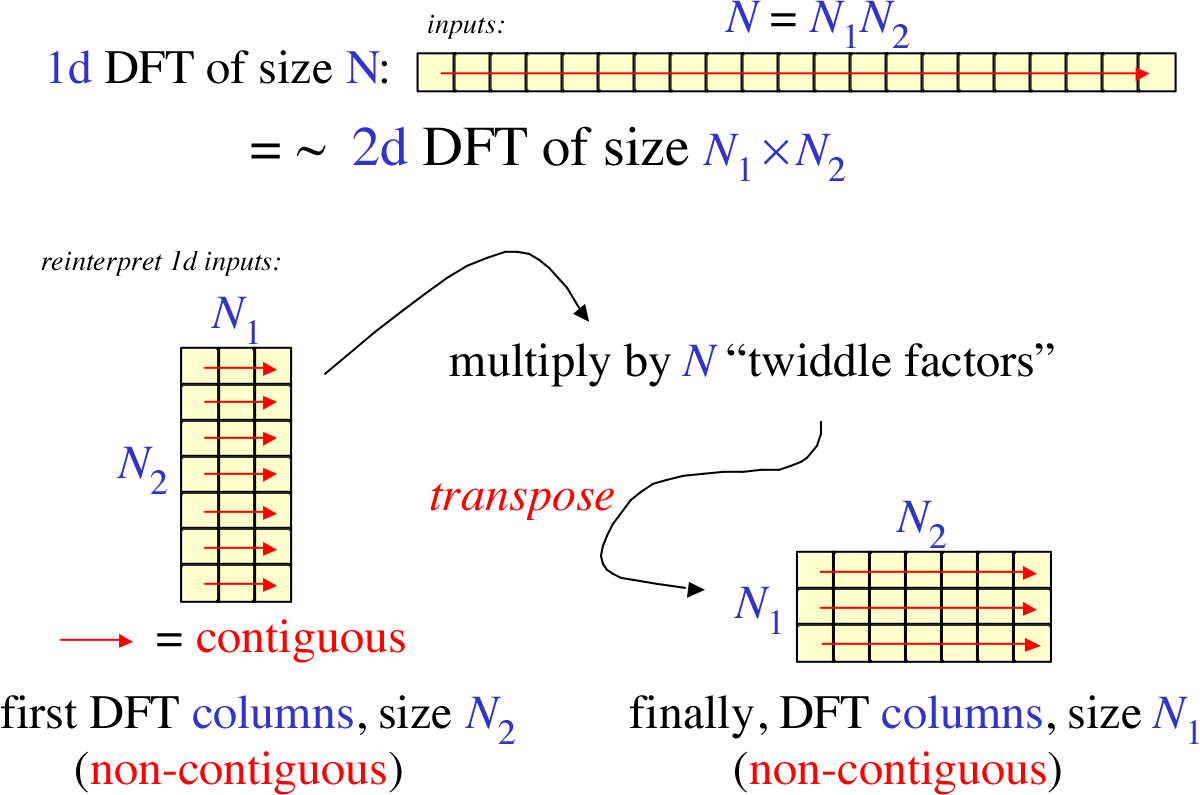
\includegraphics[scale = .6]{algorithm.png}
	\caption{Esquema representativo de los pasos asociados al algoritmo FFT, desarrollado por Cooley \cite{cooley1970fast}}
	\label{algo}
\end{figure}

\subsection{Uso de Transformadas de Fourier en digitalización de propiedades fisicoquímicas}

Diferentes enfoques han sido evaluados mediante el empleo del uso de las transformadas de Fourier en el estudio de secuencias lineales de proteínas y DNA, en particular, para el estudio de propiedades fisicoquímicas y la identificación de residuos claves asociados a peacks visuales en el espectro de frecuencia \cite{veljkovic1985possible, cosic1987prediction}. 

El uso frecuente de la digitalización, se centra principalmente en la codificación de una secuencia lineal de proteínas, en muchos casos, ha sido utilizado el potencial de interacción con electrones (PEII), ya que se han expuesto correlaciones con propensiones de moléculas orgánicas, relacionadas con toxicidad, actividad de antibióticos, carcinogenecidad, etc. \cite{veljkovic1985possible, cosic1994macromolecular, cosic1987prediction} y a partir de dicha codificación, digitalizarla para el posterior estudio de la análisis de señales.

Dichos estudios de frecuencia de señales, son componentes de modelos asociados al reconocimiento de resonancias (RRM por sus siglas en inglés), los cuales han sido estudiados en diferentes problemas del área médica, reconocimiento de Hot-spots, etc., y, en particular, enfocados en el estudio de mutaciones en proteínas \cite{cosic1994macromolecular, cosic2016analysis, cosic1987prediction}. 

Un enfoque común, asociado al estudio de señales y modelos RRM, consiste en, a partir de la secuencia lineal de residuos, emplear PEII para codificarla, a partir de su codificación, se aplica FFT como método de digitalización, para así, obtener el espectro de frecuencia y hacer los análisis de señales correspondientes \cite{veljkovic1985possible, cosic1994macromolecular, cosic2016analysis, cosic1987prediction}.

No obstante, existen otros enfoques, en donde se ha utilizado la digitalización de las propiedades fisicoquímicas como método de generación de atributos para set de datos, los cuales son sometidos a entrenamiento de predicciones, entregando medidas de desempeño satisfactorias, según los autores \cite{cadet2018application}. Sin embargo, la selección de las propiedades fisicoquímicas es arbitraria y sólo se considera la propiedad más informativa, no considerando el uso de combinaciones lineales o correlaciones entre las propiedades existentes.

Uno de los puntos relevantes, es que a partir de un conjunto de espectros de frecuencia, es posible generar un consenso y a su vez, identificar residuos relevantes al espectro y que contribuyen de manera significativa en los peaks, así como también la generación de espectros consenso a partir de secuencias diferentes, entregando uno de los principales planteamientos. \textit{Un mismo espectro de frecuencia, está asociado a una propiedad o una funcionalidad}, lo cual fue testeado en trabajos como \cite{veljkovic1985possible}. 

Esto último, lo hace una de las ventajas más relevantes para el estudio de mutaciones o reconocimiento de patrones. Sin embargo, la generalización del método ha impedido que se utilice con un mayor impacto, sólo siendo empleado en los estudios nombrados previamente. No obstante, las posibilidades de encontrar patrones o permitir modelar sistemas complejos, además de aplicar las propiedades del estudio de señales a dichos entornos de secuencias, y, las posibilidades que este método entrega para el análisis de estructuras lineales, lo hace una propuesta interesante y novedosa, que merece un esfuerzo estudiarla y aplicarla durante este trabajo de tesis.

\section{Clustering}

Clustering se define como un método de aprendizaje no supervisado, en el cual se cuenta con un conjunto de datos que representan a una muestra y en base a ésta, se trata de obtener grupos de objetos, denominados clusters \cite{jain1999data}.

Los clusters deben cumplir con dos características fundamentales:

\begin{itemize}
	\item Los objetos que pertenezcan a un mismo clúster deben ser bastante homogéneos entre ellos.
	\item Entre los clústers debe existir un alto grado de heterogeneidad.
\end{itemize}

Los métodos de clustering se tratan, fundamentalmente, de resolver el siguiente problema: Dado un conjunto de $N$ individuos, caracterizados por la información de $n$ variables $X_{j}$ con $j$ entre $1,..,n$, se plantea el reto de ser capaces de agruparlos de manera que los individuos pertenecientes a un grupo (cluster), dada la información disponible, sean tan similares entre sí como sea posible, siendo los distintos grupos entre ellos tan disimilares como sea posible.

Básicamente, el análisis constará de un algoritmo de clusterización que permitirá la obtención de una o varias particiones, de acuerdo con los criterios establecidos.

\subsection{Criterios de Similitud}

Tal como se ha mencionado anteriormente, el hecho de tener elementos pertenecientes a un mismo grupo bastante similares entre ellos y divergentes entre distintos clúster, es la característica primordial a tratar, esto último radica en la importancia de las variables que componen a un elemento en particular y en los valores que tomen éstas.

Por lo tanto se debe determinar que tan similares o diferentes son los valores que tomen las variables con respecto al elemento al cual pertenece.

Para medir lo similar o disimilar que son los individuos existe una enorme cantidad de índices de similaridad y de disimilaridad o divergencia. Todos ellos tienen propiedades y utilidades distintas y habrá que ser consciente de ellas para su correcta aplicación al momento de hacer uso de una de ellas \cite{jain1999data}.

Los índices expuestos normalmente pueden ser clasificados tal como sigue:

\begin{enumerate}
	
	\item Indicadores basados en la distancia, para lo cual se considera a los individuos como vectores en el espacio de las variables, en este sentido un elevado valor de la distancia entre dos individuos indicará un alto grado de disimilaridad entre ellos.
	
	\item Indicadores basados en coeficientes de correlación; la correlación permite indicar cuál es la fuerza y la dirección de una relación lineal entre dos variables. Se considera que dos variables cuantitativas están correlacionadas cuando los valores de una de ellas varían sistemáticamente con respecto a los valores de la otra, esto es: si se tiene dos variables (A y B) existe correlación si al aumentar los valores de A lo hacen también los de B y viceversa.
	
	\item Indicadores basados en tablas de datos de posesión o no de una serie de atributos, es decir, teniendo dos vectores A y B que representan a dos individuos de una población se hace una comparación de los elementos existentes en A y no en B, los elementos existentes en B y no en A además de la intersección entre ellos, es decir, los elementos existentes en A y en B. 
	
\end{enumerate}

\subsection{Algoritmos de Clustering}

Existen diversos algoritmos de clustering, cada uno con características que los diferencian, los cuales, pueden ser aplicados a diversos casos, dependiendo de las características de los datos de entrada, es decir, de la geometría de estos datos. Sin embargo, esta representación se basa principalmente en el uso de matrices, donde cada fila representa un ejemplo y cada columna el valor de un atributo o rasgo cualitativo para dicho ejemplo.

A continuación, se resumen algunos de los algoritmos de clustering más utilizados, explicando sus propiedades y sus características.

\subsubsection{\textit{k}-Means}

El algoritmo \textit{k}-Means, trata la separación de muestras en $ n $ grupos de igual varianza, minimizando el criterio conocido como inercia, lo que se traduce en la suma de los cuadrados dentro de los clúster \cite{arthur2007k}.

La principal característica y deficiencia a la vez, es que se requiere que el número de grupos sea entregado, es decir, se debe entregar el valor de $k$, así, si se selecciona un valor de $k = 3$, serán tres grupos los que se encontrarán. 

Este algoritmo divide un set de $N$ ejemplos $X$ en $K$ particiones distintas denominadas clúster $C$, cada uno de ellos descrito por la media $\mu_{j}$ de las muestras en el clúster. Esta media es llamada centroide, por lo que en general, \textit{k}-means  elige sus centroides de tal manera que el principio de inercia sea reducido al mínimo, es decir, que la suma de los cuadrados de los integrantes de un mismo grupo sea mínima, a través de:

\begin{equation}
	\sum_{i=0}^{n} \min_{\mu_{j} \in C} (|| x_{j}-\mu_{i}||^{2})
\end{equation}

Sin embargo, el principio de inercia, o la suma de los cuadrados mínimos entre los integrantes de los clustering, puede sufrir varios inconvenientes:

\begin{itemize}
	\item Se hace la suposición de que las agrupaciones son convexas e isotrópicas, lo cual no se da siempre, razón por la que responde mal ante a clusters que posean forma alargadas o con formas irregulares.
	
	\item No es una métrica normalizada, es decir, se sabe que los valores más bajos son mejores y el cero es óptimo. Sin embargo, en espacios de muy de alta dimensionalidad, las distancias euclidianas tienden a ser infladas, lo que se conoce como  "la maldición de la dimensionalidad", razón por la cual, son utilizados algoritmos de reducción de la dimensionalidad, tal como PCA.
	
\end{itemize}

Ambos puntos, son posibles observarlos en la Figura  \ref{kerror}, en la cual se exponen, problemas con varianzas distintas, diferencias asociadas al tamaño de los clúster, anisotropía\footnote{Las variables varían en base a las direcciones en las que se examinan} de los datos, etc.

\begin{figure}[!h]
	
	\centering
	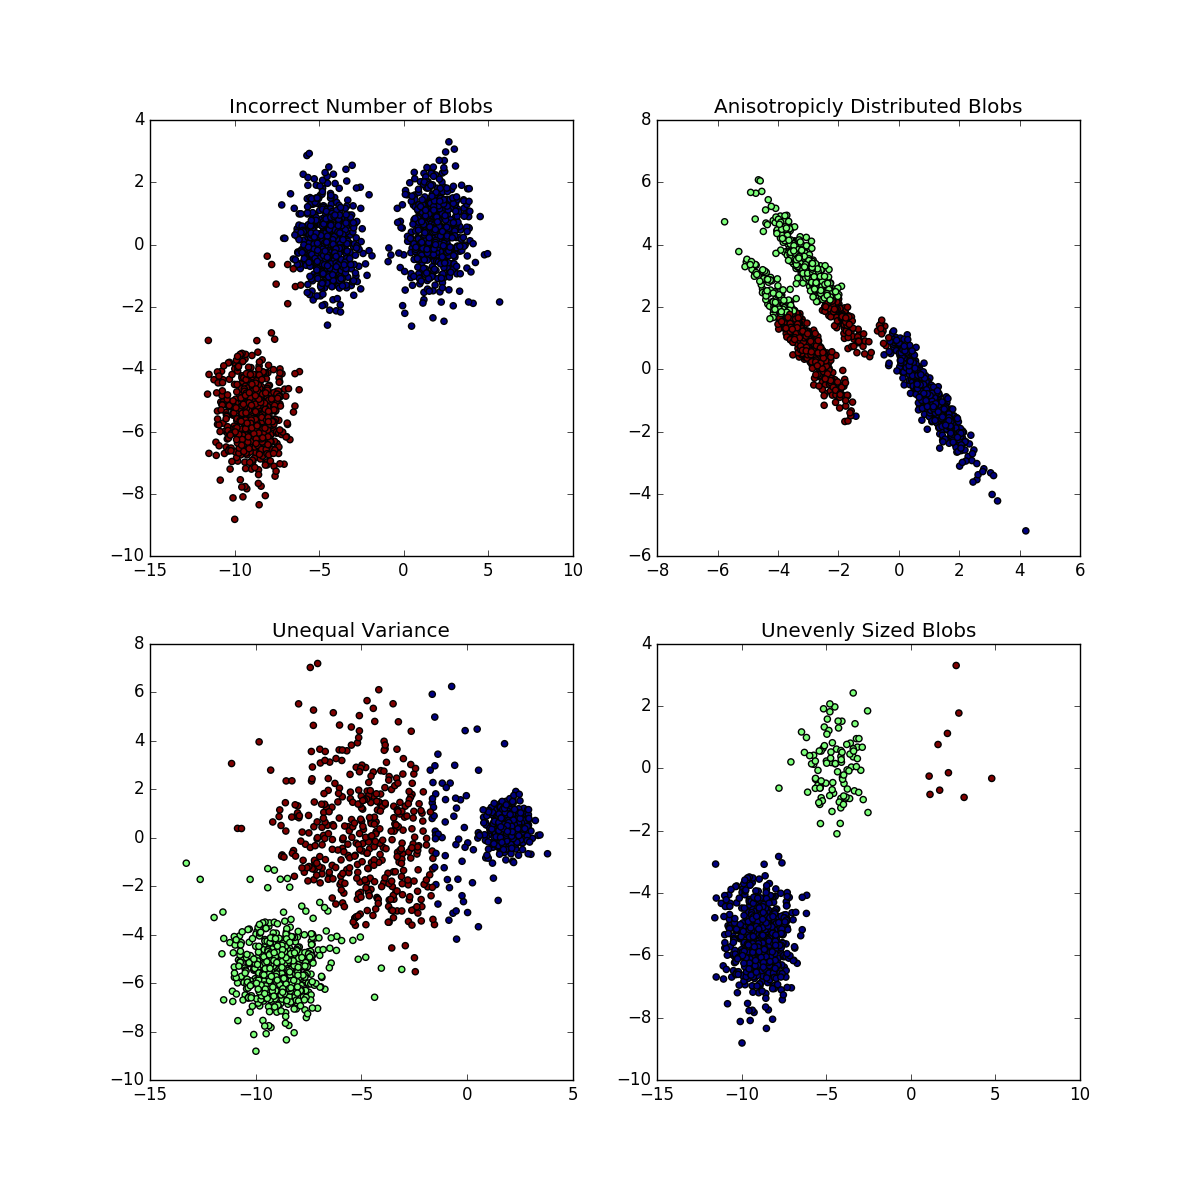
\includegraphics[scale = .4]{kmeansError.png}
	\caption{Posibles inconvenientes con los datos, donde k-medias  no funciona correctamente}
	\label{kerror}
\end{figure}


En términos básicos, el algoritmo tiene tres pasos. El primer paso consiste en elegir los centroides iniciales, con el método más básico para elegir $k$ muestras del conjunto de datos $X$. Después de la inicialización, \textit{k}-means  consta de un bucle entre los otros siguientes dos pasos. 

En una primera instancia, asigna cada muestra a su centroide más cercano. Posterior a ello, se crean nuevos centroides tomando el valor medio de todas las muestras asignadas a cada centroide anterior. La diferencia entre la media anterior y la actual (diferencia entre centroides) se calcula y se itera estas acciones hasta que este valor sea inferior a un umbral. En otras palabras, se repite hasta que los centroides no se mueven de manera significativa.

\subparagraph{Clustering Jerarquizado\\\\}

Clustering jerárquico o HCA (por sus siglas en inglés) es un método de análisis de conglomerados, que busca construir una jerarquía de agrupaciones. Las estrategias para la agrupación son posible dividirlas en dos \cite{johnson1967hierarchical}:

\begin{itemize}
	
	\item \textbf{Aglomerativa}: consiste en un enfoque de "abajo hacia arriba": cada observación se inicia en su propio clúster, y pares de grupos se fusionan a medida que se asciende en la jerarquía. 
	
	\item \textbf{Divisiva}: consiste en un enfoque "de arriba hacia abajo": todas las observaciones se inician en un único clúster, y las divisiones se realizan de forma recursiva conforme se desciende en la jerarquía.
	
\end{itemize}

Siendo generalmente expuestos los resultados en forma de dendrograma \cite{sokal1962comparison}, por otro lado, la complejidad del algoritmo, en el caso general es $\displaystyle O(n^{2}\log(n))$, lo cual presenta problemas para set de datos extensos.

Con el fin de decidir qué grupos se deben combinar (por aglomeración), o cuando un grupo se debe dividir (por división), se requiere una medida de disimilitud entre los conjuntos de observaciones. En la mayoría de los métodos de agrupación jerárquica, esto se logra mediante el uso de una métrica apropiada (una medida de la distancia entre pares de observaciones), y un criterio de vinculación que especifica la disimilitud de conjuntos como una función de las distancias por pares de observaciones en los conjuntos.

Las métricas asociadas pueden son las mismas utilizadas en el algoritmo $k$-means y las aplicadas en el método KNN de aprendizaje supervisado.


El criterio de linkage determina la distancia entre conjuntos de observaciones como una función de las distancias por pares entre observaciones.

Algunos criterios de linkage de uso común entre los dos conjuntos de observaciones $A$ y $B$ son expuestos en la tabla \ref{tab:summary-linkage}.

% Please add the following required packages to your document preamble:
% \usepackage{longtable}
% Note: It may be necessary to compile the document several times to get a multi-page table to line up properly
\begin{longtable}[c]{|l|l|}
	\hline
	\multicolumn{2}{|c|}{\textbf{Criterios de linkage comunes en métodos HCA}} \\ \hline
	\endfirsthead
	%
	\endhead
	%
	\textbf{Complete linkage clustering} & $ \max \,\{\,d(a,b):a\in A,\,b\in B\,\}.$ \\ \hline
	\textbf{Single-linkage clustering} & $ \min \,\{\,d(a,b):a\in A,\,b\in B\,\}.$ \\ \hline
	\textbf{Average linkage clustering} & $ {\frac {1}{||A||B||}}\sum _{{a\in A}}\sum _{{b\in B}}d(a,b).$ \\ \hline
	\textbf{Centroid linkage clustering} & ${\displaystyle \|c_{s}-c_{t}\|}$ con ${\displaystyle c_{s}}$ y $c_{t}$ centroides \\ \hline
	\textbf{Minimum energy clustering} & $ {\frac {2}{nm}}\sum _{{i,j=1}}^{{n,m}}\|a_{i}-b_{j}\|_{2}-{\frac {1}{n^{2}}}\sum _{{i,j=1}}^{{n}}\|a_{i}-a_{j}\|_{2}-{\frac {1}{m^{2}}}\sum _{{i,j=1}}^{{m}}\|b_{i}-b_{j}\|_{2}.$ \\ \hline
	\caption{Resumen de linkages comunes utilizados en métodos de clustering jerárquicos.}
	\label{tab:summary-linkage}\\
\end{longtable}

Un aspecto interesante de este algoritmo es que pueden ser añadidas las limitaciones de conectividad, es decir, sólo grupos adyacentes pueden fusionarse entre sí, esto es, a través de una matriz de conectividad que define para cada muestra, las muestras de vecinos después de una estructura dada de los datos. Estas restricciones son útiles para imponer una cierta estructura local, así como para hacer que el algoritmo sea más rápido, especialmente cuando el número de las muestras es alta.

\subsubsection{Affinity Propagation}

AffinityPropagation crea grupos mediante el envío de mensajes entre pares de muestras hasta la convergencia. Un conjunto de datos es descrito por el uso de un pequeño número de ejemplares, que se identifican como las más representativas de otras muestras. Los mensajes enviados entre pares representan la idoneidad para una muestra a ser el ejemplo de la otra, la cual se actualiza en respuesta a los valores de otros pares. Esta actualización ocurre de forma iterativa hasta la convergencia, momento en el que se eligen los ejemplares finales, y por lo tanto se da el agrupamiento final \cite{frey2007clustering}.

Se elige el número de grupos en base a los datos proporcionados. Para este propósito, los dos parámetros importantes son la preferencia, que controla el número de ejemplares que se utilizan, y el factor de amortiguamiento.

El principal inconveniente que presenta este algoritmo viene dado por la complejidad que posee, el cual se representa por $O(N^{2}T)$, donde $N$ es el número de muestras y $T$ es el número de operaciones necesarias para converger, razón por la cual, el uso de este algoritmo es para set de datos con pequeña cantidad de ejemplos.

Con respecto a la descripción del algoritmo, es posible mencionar que los mensajes enviados a los grupos, pertenecen a dos categorías, la primera es la responsabilidad $r(i,k)$ la cual consiste en la evidencia acumulada que denota que la muestra $k$ podría ser un ejemplar para la muestra $i$. La segunda es la disponibilidad $a(i,k)$, la cual se define como la evidencia existente para que la muestra $i$ pueda escoger a la muestra $k$ para ser su ejemplar, además considera todos los valores de las otras muestras de $k$ que podrían ser ejemplares. De esta manera, los ejemplares son escogidos por las muestras si:

\begin{itemize}
	
	\item Existe una similaridad bastante alta con respecto a las muestras.
	
	\item Si es elegido por muchas muestras y resulta ser representativo de sí mismos.
\end{itemize}

En forma matemática es posible definir la responsabilidad como:

\begin{equation}	
	r(i, k) \leftarrow s(i, k) - max [ a(i, \acute{k}) + s(i, \acute{k}) \forall \acute{k} \neq k ]
\end{equation}

Donde $s(i,k)$ es la similaridad entre las muestras $i$ y $k$. 

A su vez, la disponibilidad, es posible definirla como:

\begin{equation}
	a(i, k) \leftarrow min [0, r(k, k) + \sum_{\acute{i}~s.t.~\acute{i} \notin \{i, k\}}{r(\acute{i}, k)}]
\end{equation}

\subsubsection{Mean Shift}

El algoritmo de Mean Shift tiene como objetivo descubrir manchas (blobs) en una densidad uniforme de las muestras. Es un algoritmo basado en centroides, que funciona mediante la actualización de los candidatos para centroides para ser la media de los puntos dentro de una región determinada. Estos candidatos se filtran en una etapa de post-procesamiento para eliminar duplicados y así formar el conjunto final de centroides \cite{cheng1995mean}.

Dado un candidato $x_{i}$ para la iteración $t$, el candidato a centroide es actualizado en base a la ecuación:

\begin{equation}
	x_i^{t+1} = x_i^t + m(x_i^t)
\end{equation}

Donde $N (x_i)$ es la vecindad de las muestras dentro de una distancia dada alrededor $x_i$ y $m$ es el vector de desplazamiento medio, que se calcula para cada centroide que apunta hacia una región del aumento máximo en la densidad de puntos. Ésta se calcula utilizando la siguiente ecuación, en la que la actualización de manera efectiva denota a un centroide ser la media de las muestras dentro de su vecindad:

\begin{equation}		
	m(x_i) = \frac{\sum_{x_j \in N(x_i)}K(x_j - x_i)x_j}{\sum_{x_j \in N(x_i)}K(x_j - x_i)}
\end{equation}

Algunas de las características de Mean Shift, son

\begin{itemize}
	
	\item Ajusta automáticamente el número de grupos, dependiendo de un parámetro bandwidth, el cual se asocia al tamaño de la región en la que se debe buscar los centroides. 
	
	\item No es altamente escalable, ya que requiere múltiples búsquedas de vecinos más cercanos durante la ejecución del algoritmo. 
	
	\item Garantiza convergencia, deteniendo la iteración cuando el cambio en centroides es pequeño.
		
\end{itemize}

\subsubsection{DBSCAN}

El algoritmo DBSCAN ve agrupaciones como áreas de alta densidad separadas por zonas de baja densidad. Debido a esta visión bastante genérica, las agrupaciones que se encuentran pueden ser de cualquier forma, en lugar de \textit{k}-means  que supone que los grupos tienen la forma convexa \cite{tran2013revised}.

El componente central de DBSCAN es el concepto de muestras de núcleo, las cuales son las muestras que se encuentran en áreas de alta densidad. Por lo tanto, un clúster es un conjunto de muestras de núcleos, cada uno cerca del otro (medido por alguna medida de distancia) y un conjunto de muestras no básicas que se encuentran cerca de una muestra básica. Hay dos parámetros necesarios para el algoritmo, min samples y EPS, los cuales definen formalmente la densidad deseada \cite{tran2013revised}.


Más formalmente, se define una muestra del núcleo como una muestra del conjunto de datos de tal manera que existe una cantidad de muestra mínimas y a su vez otras muestras dentro de una distancia de EPS, que se definen como vecinos de la muestra del núcleo. Esto dice que la muestra de núcleo se encuentra en un área densa del espacio vectorial. Un clúster es un conjunto de muestras de núcleo que se puede construir mediante la adopción de forma recursiva de una muestra básica, la búsqueda de todos sus vecinos que son muestras de la base, la búsqueda de la totalidad de sus vecinos que son muestras de núcleo, y así sucesivamente. Un cluster también tiene un conjunto de muestras no básicas, que son las muestras que son vecinos de una muestra básica de la agrupación, pero no son en sí mismos muestras de núcleos. Intuitivamente, estas muestras están al margen de un clúster.


Cualquier muestra de núcleo es parte de un clúster, por definición. Cualquier muestra que no es una muestra del núcleo, y está al menos una distanca eps de cualquier muestra del núcleo, se considera un valor atípico por el algoritmo.

Normalmente, los resultados del algoritmo, pueden representarse tal como se expone en la Figura  \ref{dbscanE}, el color indica la pertenencia al clúster, con grandes círculos que indican muestras de núcleos encontrados por el algoritmo, círculos más pequeños son muestras no básicas que todavía son parte de un clúster. Por otra parte, los valores atípicos se indican con puntos negros.

\begin{figure}[!h]
	\centering
	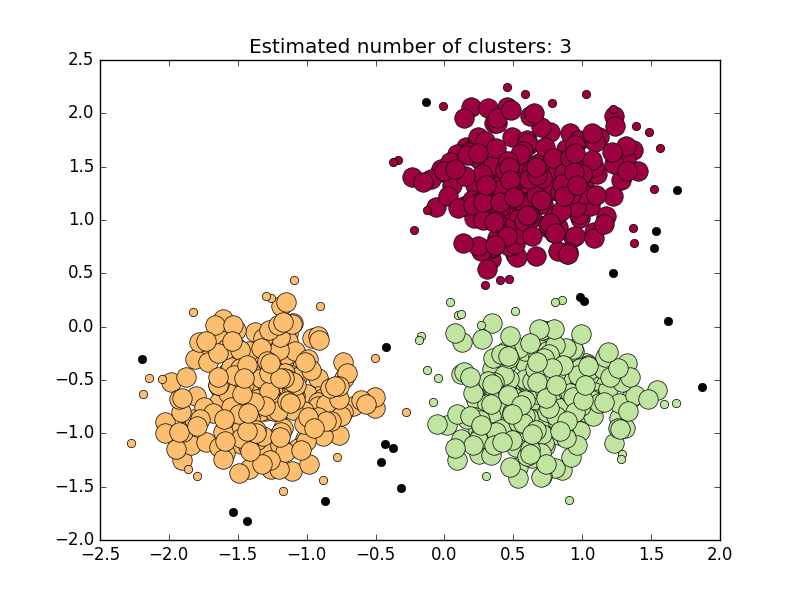
\includegraphics[scale=.4]{DBSCANexampl.png}
	\caption{Representación de resultados al aplicar la clusterización por DBSCAN}
	\label{dbscanE}
\end{figure}

\subsubsection{Birch}

Birch construye un árbol llamado Characteristic Feature Tree (CFT) de los datos correspondientes. Los datos están esencialmente con pérdida de información, comprimidos en un conjunto de nodos de rasgo característico denominados CF nodos. Estos tienen una serie de subgrupos llamados subclusters de rasgo característico, ubicados en los nodos CF no terminales los cuales pueden tener CF nodos como hijos \cite{zhang1997birch}.

Los subgrupos CF pueden contener la información necesaria para la agrupación que evite la necesidad de mantener los datos de entrada enteros en la memoria. Esta información incluye:

\begin{itemize}
	
	
	\item Número de muestras en un subgrupo.
	\item Suma lineal, representada por un vector n-dimensional que sostiene la suma de todas las muestras.
	\item Suma al cuadrado, representada por la suma cuadrática de la norma L2 de todas las muestras.
	\item Centroides, para evitar un nuevo cálculo de sumas lineales con respecto al número de muestras.
	\item Norma al cuadrado de los centroides.
	
\end{itemize}

El algoritmo de Birch tiene dos parámetros, el umbral y el factor de branching. El factor de branching limita el número de subgrupos en un nodo y el umbral limita la distancia entre la muestra de entrada y los subclusters existentes.

Este algoritmo puede ser visto como un método de instancia o reducción de datos, ya que reduce los datos de entrada a un conjunto de subclusters que se obtienen directamente de las hojas de la CFT. Estos datos reducidos pueden ser procesados por la alimentación en un clúster global. Este clúster global puede ser establecido por $n$ clusters. Si este parámetro se establece como valor 0 o ninguno, los subgrupos de las hojas se leen directamente, de lo contrario un paso global de la agrupación etiqueta estos subgrupos en grupos globales y las muestras se asignan a la etiqueta global del subgrupo más cercano.

Una descripción del algoritmo, es posible realizarla en los siguientes puntos:

\begin{itemize}
	
	\item Una nueva muestra se inserta en la raíz del árbol CF que es un nodo CF. A continuación, se fusiona con el subgrupo de la raíz, el que tiene el radio más pequeño después de la fusión, limitada por el umbral de ramificación y condiciones de los factores. Si el subcluster tiene algún nodo hijo, entonces esto se realiza repetidamente hasta que llega a una hoja. Después de encontrar el subcluster más cercano en la hoja, las propiedades de este subgrupo y los subclusters padres se actualizan de forma recursiva.
	
	\item Si el radio del subcluster obtenido mediante la fusión de la nueva muestra y el subgrupo más cercano es mayor que el cuadrado del umbral y si el número de subclusters es mayor que el factor de ramificación, a continuación, un espacio se asigna temporalmente a esta nueva muestra. Los dos subgrupos más lejanos se toman y de los subgrupos se dividen en dos grupos sobre la base de la distancia entre estos subgrupos.
	
	\item Si este nodo de división tiene un subgrupo de los padres y no hay espacio para un nuevo subgrupo, entonces el padre se divide en dos. Si no hay espacio, entonces este nodo se divide de nuevo en dos y el proceso se continúa de forma recursiva, hasta que llega a la raíz
	
\end{itemize}

\subsubsection{Mixture Model}

Los métodos de clustering basado en modelos tratan de optimizar el conjunto de datos a un modelo
matemático. En general estos métodos se basan en la suposición que los datos han sido generados por una mezcla de distribuciones de probabilidad. Dentro de los más utilizados se encuentran \textbf{Gaussian Mixture} \cite{zivkovic2004improved} y \textbf{Expectation-Maximization} \cite{moon1996expectation}.

Expectation Maximization, supone que los datos emergen de una mecla de distribuciones, donde cada distribución se denomina como \textit{component distribution}, razón por la cual, los datos pueden agruparse usando un modelo de mezcla de densidades de $k$ distribuciones de probabilidades. Sin embargo, el problema reside en estimar los parámetros de estas distribuciones para proveer del mejor ajuste posible a los datos \cite{moon1996expectation}. 

El algoritmo Expectation Maximization (EM) puede ser considerado como una extensión de \textit{k}-means, esto es debido a que: Si \textit{k}-means asigna cada objeto a un clúster en función de su media, EM asigna cada objeto a un clúster en función de un peso que representa la probabilidad de pertenencia al clúster. Esto requiere que se defina una distribución de probabilidad para los clusters.

Por otro lado, un modelo de mezcla gaussiano como Gaussian Mixture Model (GMM) es una función de densidad de probabilidad representada por una suma de componentes gausianas, GMMs son usadas como modelos paramétricos de la distribución de probabilidad de medidas continuas, donde los parámetros de GMM son estimados usando iterativamente el algoritmo Expectation-Maximization \cite{zivkovic2004improved}.

Un GMM es una suma con pesos de densidades gaussianas:

\begin{equation}	
	p(\vec{x}) = \sum_{i=1}^{M} w_i \times N(\vec{x}|\mu_i, \sum_{i})
\end{equation}

Donde $\vec{x}$ es un vector D-dimensional de datos, $w_i$ son los pesos con $\sum_{i=1}^{M} w_i = 1$, y $N(\vec{x}|\mu_i, \sum_{i})$ es la densidad gaussiana, por lo tanto, la caracterización se completa con la media, la matríz de covarianza y el peso de cada componente gaussiana.

Una de las limitantes es que el número de componentes gausianos tiene que ser fijado al principio
del algoritmo.

El GMM consta de los siguientes pasos:

\begin{enumerate}
	
	\item \textbf{Iniziacilización}: para cada clase, un vector compuesto de la media y la matriz de covarianza es construido. Este vector representa las características de la distribución gaussiana usada para caracterizar las entidades del conjunto de datos. Inicialmente estos valores son generados aleatoreamente, posteriormente el algoritmo EM trata de aproximar los valores del vector de la distribución real de los datos. 
	
	\item Se estima la probabilidad de cada elemento de pertenecer a un clúster.
	
	\item Se estiman los parámetros de la distribución de probabilidad para el próximo ciclo, primero se calcula la media de la clase a través de la media de todos los puntos en función del grado de relevancia de cada punto, continuando con el cálculo de la matriz de covarianza.
	
	\item \textbf{Convergencia}: Después de cada ciclo se ejecuta un test de convergencia para verificar cuánto ha cambiado el vector de parámetros y si la diferencia es menor que un umbral de tolerancia el algoritmo se detiene, no obstante es posible detener el algoritmo debido al alcance de un número máximo de ciclos.
	
\end{enumerate}

Una representación visual del modelo es posible observarla en la Figura  \ref{esquemaR}, en ella se aprecia cómo a medida que se va iterando el algoritmo se generan los cambios y las \textit{separaciones} en grupos de clúster definidos.

\begin{figure}[!h]
	
	\centering
	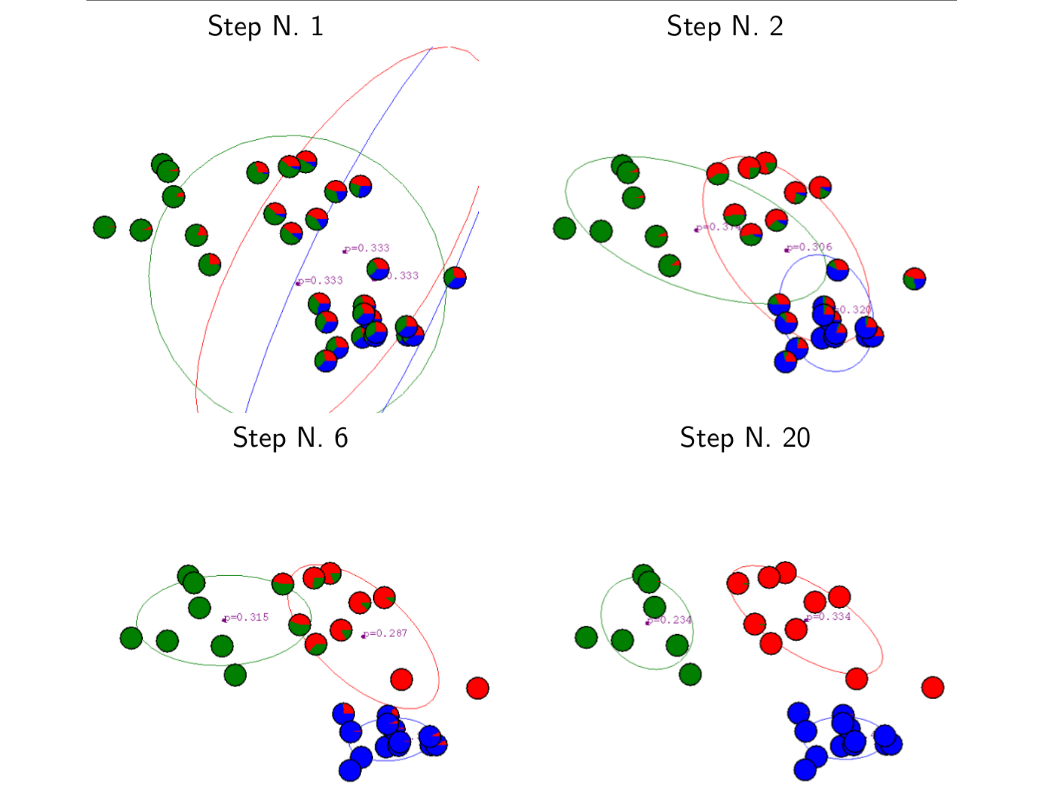
\includegraphics[scale=.4]{pasosGMM.png}
	\caption{Esquema representativo de cambios durante las iteraciones en GMM}
	\label{esquemaR}
\end{figure}

\subsubsection{Cuadro Resumen}

En la Tabla \ref{cuadroResumen} se expone un resumen de las características de cada algoritmo expuesto, la escalabilidad que poseen, las distancias que ocupan, los casos de uso y los parámetros que poseen.

\begin{table}[]
	\centering
	\begin{tabular}{|l|l|l|l|l|}
		\hline
		\multicolumn{5}{|c|}{\textbf{Tabla resumen de Algoritmos de Aprendiza No Supervisado}}                                                                                                                                                                                                                                                                                                                                                                                                                                          \\ \hline
		\textbf{Algoritmo}                                                                  & \textbf{Parámetros}                                                                       & \textbf{Escalabilidad}                                                                                  & \textbf{Usos}                                                                                                                                 & \textbf{Métrica usada}                                                              \\ \hline
		\textbf{K-Means}                                                                    & \begin{tabular}[c]{@{}l@{}}Número de \\ clúster\end{tabular}                              & \begin{tabular}[c]{@{}l@{}}Muchas muestras, \\ mediana cantidad\\ de clúster.\end{tabular}              & \begin{tabular}[c]{@{}l@{}}De propósito\\ general, la \\ geometría plana, \\ no demasiados \\ grupos\end{tabular}                             & \begin{tabular}[c]{@{}l@{}}Distancia entre\\ puntos\end{tabular}                    \\ \hline
		\textbf{\begin{tabular}[c]{@{}l@{}}Affinity \\ propagation\end{tabular}}            & preferencia                                                                               & \begin{tabular}[c]{@{}l@{}}No escalable con \\ n ejemplos\end{tabular}                                  & \begin{tabular}[c]{@{}l@{}}Muchos clúster, \\ tamañode clúster \\ desigual, \\ geometría no \\ plana\end{tabular}                             & \begin{tabular}[c]{@{}l@{}}Distancia\\ gráfica\end{tabular}                         \\ \hline
		\textbf{Mean-shift}                                                                 & bandwidth                                                                                 & \begin{tabular}[c]{@{}l@{}}No escalable con \\ n ejemplos\end{tabular}                                  & \begin{tabular}[c]{@{}l@{}}Muchos clúster, \\ tamañode clúster \\ desigual, geometría \\ no plana\end{tabular}                                & \begin{tabular}[c]{@{}l@{}}Distancia entre\\ puntos\end{tabular}                    \\ \hline
		\textbf{\begin{tabular}[c]{@{}l@{}}Ward \\ hierarchical \\ clustering\end{tabular}} & \begin{tabular}[c]{@{}l@{}}Número de \\ clúster\end{tabular}                              & \begin{tabular}[c]{@{}l@{}}Mucha cantidad \\ de ejemplos y de \\ clusters\end{tabular}                  & \begin{tabular}[c]{@{}l@{}}Cualquier clúster, \\ es posible \\ conección de \\ constraints\end{tabular}                                       & \begin{tabular}[c]{@{}l@{}}Distantia entre\\ puntos\end{tabular}                    \\ \hline
		\textbf{\begin{tabular}[c]{@{}l@{}}Agglomerative \\ clustering\end{tabular}}        & \begin{tabular}[c]{@{}l@{}}Número de \\ clúster, tipo de \\ unión, distancia\end{tabular} & \begin{tabular}[c]{@{}l@{}}Mucha cantidad\\ de ejemplos y de\\ clusters\end{tabular}                    & \begin{tabular}[c]{@{}l@{}}Muchos clusters, \\ posiblemente \\ restricciones de \\ conectividad, \\ distancias \\ no euclidianas\end{tabular} & \begin{tabular}[c]{@{}l@{}}Cualquier \\ distancia pairwise\end{tabular}             \\ \hline
		\textbf{DBSCAN}                                                                     & tamaño vecino                                                                             & \begin{tabular}[c]{@{}l@{}}Mucha cantidad \\ de ejemplos, \\ mediana\\ cantidad de clúster\end{tabular} & \begin{tabular}[c]{@{}l@{}}Geometría no plana, \\ tamaños de clusters \\ distintos\end{tabular}                                               & \begin{tabular}[c]{@{}l@{}}Distancia entre\\ puntos vecinos\end{tabular}            \\ \hline
		\textbf{\begin{tabular}[c]{@{}l@{}}Gaussian \\ mixtures\end{tabular}}               & variado                                                                                   & No escalable                                                                                            & \begin{tabular}[c]{@{}l@{}}Geometría plana, \\ bueno para la \\ estimación de la \\ densidad\end{tabular}                                     & \begin{tabular}[c]{@{}l@{}}Distancia \\ Mahalanobis para\\ los centros\end{tabular} \\ \hline
		\textbf{Birch}                                                                      & \begin{tabular}[c]{@{}l@{}}branching, \\ umbral\end{tabular}                              & \begin{tabular}[c]{@{}l@{}}Alto número de\\ clúster y ejemplos\end{tabular}                             & \begin{tabular}[c]{@{}l@{}}Largo set de datos, \\ eliminación valores \\ atípicos, \\ reducción de datos\end{tabular}                         & \begin{tabular}[c]{@{}l@{}}distancia \\ euclidiana\\ entre puntos\end{tabular}      \\ \hline
	\end{tabular}
	
	
	\caption{Cuadro resumen de algoritmos de aprendizaje supervizado}
	\label{cuadroResumen}
\end{table}

\subsubsection{Evaluación del desempeño de un clustering}\label{evaluacion}

Evaluar el desempeño de un algoritmo de clustering no es tan trivial como contar el número de errores o la precisión y la recuperación de un algoritmo de clasificación supervisada. En particular, cualquier métrica de evaluación no debe tomar los valores absolutos de las etiquetas de clúster en cuenta, sino más bien si estas agrupaciones definen separaciones de los datos, de tal manera que los miembros que pertenecen a la misma clase son más similares que los miembros de diferentes clases de acuerdo con alguna similitud métrica.

Existen diversas medidas de similitud con el fin de evaluar el clustering, las cuales se explican a continuación:

\subparagraph{Adjusted Rand index\\\\}

Dado el conocimiento de las clases asignadas como verdaderas (etiquetas verdaderas) y las etiquetas obtenidas por el algoritmo de clustering (etiquetas predichas) el adjuster rand index es una función que mide la similaridad de las dos asignaciones, ignorando permutaciones, posee valores entre -1 y 1, siendo 1 el valor perfecto. Sin embargo, es imperante para evaluar el desempeño, conocer las etiquetas verdaderas de los datos \cite{yeung2001details}.

Matemáticamente es posible definirlo como:

Sea $C$ una asignación de clase real y dada la agrupación $K$, se define $a$ y $b$ como:

\begin{itemize}
	
	\item $a$, el número de pares de elementos que estan en el mismo set en $C$ y en el mismo set en $K$.
	\item $b$, el número de pares de elementos que estan en diferentes set en $C$ y en diferentes set en $K$.
\end{itemize}

El valor del rand index no ajustado viene dado por:

\begin{equation}
	RI = \frac{a + b}{C_2^{n_{samples}}}
\end{equation}

Donde $C_2^{n_{samples}}$ es el número total de posibles pares en el set de datos.

Sin embargo, la puntuación de RI no garantiza que las asignaciones de etiquetas al azar conseguirán un valor cercano a cero, para contrarrestar este efecto se puede descartar la esperanza RI $E[RI]$ de etiquetas al azar mediante la definición del adjusted rand index:

\begin{equation}
	ARI = \frac{RI - E[RI]}{\max(RI) - E[RI]}	
\end{equation}

\subparagraph{Información mutua basada en scores\\\\}

Dado el conocimiento de las etiquetas de las clases reales y las asignaciones obtenidas de algoritmos de agrupación de las mismas muestras, el mutual information es una función que mide el \textit{acuerdo} de las dos asignaciones, ignorando las permutaciones. Existen dos versiones normalizadas diferentes de esta medida:

Normalized Mutual Information, NMI (Información mutua normalizada) y Adjusted Mutual Information, AMI (Información mutua ajustada). NMI es a menudo usado en la literatura mientras que AMI fue porpuesto más recientemente \cite{peng2005feature}.

Matemáticamente, es posible definir esta forma de evaluación tal que: se asume dos etiquetas asignadas (de los mismos $N$ objetos), $U$ y $V$, su entropía es la cantidad de incertidumbre para un conjunto de particiones definido por:

\begin{equation}
	H(U) = \sum_{i=1}^{|U|}P(i)\log(P(i))
\end{equation}

donde $P(i) = |U_i| / N$ es la probabilidad que un objecto seleccionado aleatoriamente de la clase $U$ sea asignado a la clase $U_i$, de igual manera para $V$:

\begin{equation}	
	H(V) = \sum_{j=1}^{|V|}P'(j)\log(P'(j))
\end{equation}

Con $P'(j) = |V_j| / N$ el mutual information (MI) entre $U$ y $V$ es calculado por:

\begin{equation}	
	MI(U, V) = \sum_{i=1}^{|U|}\sum_{j=1}^{|V|}P(i, j)\log(\frac{P(i,j)}{P(i)P'(j)})
\end{equation}

donde $P(i, j) = |U_i \cap V_j| /N$ es la probabilidad de que un objeto seleccionado aleatoriamente sea asignado a ambas clases $U_i$ y $V_j$.

El valor normalizado del mutual information es definido como:

\begin{equation}	
	NMI(U, V) = \frac{MI(U, V)}{\sqrt{H(U)H(V)}}
\end{equation}
Este valor del mutual information y también la variante normalizada no se ajusta al azar y tiende a aumentar a medida que aumenta el número de diferentes etiquetas (clusters), independientemente de la cantidad real de \textit{mutual information} entre las asignaciones de etiquetas.

El valor esperado para el mutual information puede ser calculado usando la ecuación descrita por  Vinh, Epps, and Bailey, (2009). En esta ecuación, $a_i = |U_i|$ (el número de elementos en $U_i$) y $b_j = |V_j|$ (el número de elementos en $V_j$).
\begin{equation}	
	E[MI(U,V)]=\sum_{i=1}^{|U|} \sum_{j=1}^{|V|} \sum_{n_{ij}=(a_i+b_j-N)^+ }^{\min(a_i, b_j)} \frac{n_{ij}}{N}\log ( \frac{ N.n_{ij}}{a_i b_j}) \frac{a_i!b_j!(N-a_i)!(N-b_j)!}{N!n_{ij}!(a_i-n_{ij})!(b_j-n_{ij})! (N-a_i-b_j+n_{ij})!}	
\end{equation}

Usando el valor esperado, el adjusted mutual information puede ser calculado usando una forma similar al ARI:

\begin{equation}	
	AMI = \frac{MI - E[MI]}{\max(H(U), H(V)) - E[MI]}
\end{equation}

\subparagraph{Homogeneidad, Completación y V-measure \\\\}

Para el caso en el que se conozca a ciencia cierta las etiquetas reales de las clases, es posible definir medidas de evaluación basándose en la entropía existente. En particular Rosenberg y Hirschberg (2007) \cite{rosenberg2007v} definen los siguientes dos objetivos deseables para cualquier asignación de clusters:

\begin{itemize}
	
	\item \textbf{homogeneidad}: cada clúster contiene sólo miembros de una única clase.
	
	\item \textbf{Totalidad (completeness)}: todos los miembros de una clase son asignados a un mismo clúster.
	
\end{itemize}

Los valores de estos score abarcan los rangos entre 0 y 1, siendo 1 el score perfecto.

Es posible definir la homogeneidad y el completeness como $h$ y $c$, respectivamente:

\begin{equation}	
	h = 1 - \frac{H(C|K)}{H(C)}	
\end{equation}

\begin{equation}
	c = 1 - \frac{H(K|C)}{H(K)}
\end{equation}

donde $H(C|K)$ es la entropía condicional de las clases dada la asignación del clúster y es definida por:

\begin{equation}	
	H(C|K) = - \sum_{c=1}^{|C|} \sum_{k=1}^{|K|} \frac{n_{c,k}}{n} \cdot \log(\frac{n_{c,k}}{n_k})
\end{equation}

y $H(C)$ es la entropía de la clase y cuyo valor viene dado por:

\begin{equation}	
	H(C) = - \sum_{c=1}^{|C|} \frac{n_c}{n} \cdot \log(\frac{n_c}{n})
\end{equation}

con $n$ siendo el número total de muestras, $n_c$ y $n_k$ el número de muestras respectivamente pertenecientes a la clase $c$ y al clúster $k$, y finalmente $n_{c,k}$ el número de muestra de la clase $c$ asignados al clúster $k$.

Rosenberg y Hirschberg \cite{rosenberg2007v} también definieron un \textbf{V-measure} como el score medio de la homogeneidad y completeness:

\begin{equation}	
	v = 2 \cdot \frac{h \cdot c}{h + c}
\end{equation}

\subparagraph{Silhouette Coefficient\\\\}

Este coeficiente es posible utilizarlo cuando se desconocen las reales etiquetas de los ejemplos, una puntuación alta (por sobre 0.75) denota un modelo con grupos bien definidos \cite{rousseeuw1987silhouettes}. Este coeficiente se define para cada muestra y posee dos score:

\begin{itemize}
	
	\item \textbf{a}: la distancia media entre un ejemplo y todos los otros puntos en la misma clase.
	
	\item \textbf{b}: la distancia media entre un ejemplo y todos los otros puntos en el siguiente clúster vecino.
\end{itemize}

El coeficiente para una única muestra, viene dado por:

\begin{equation}	
	s = \frac{b - a}{max(a, b)}
\end{equation}

\subparagraph{Calinski-Harabaz Index\\\\}

Este índice es utilizado cuando las etiquetas son desconocidas, donde un mayor valor de éste implica un modelo mejor definido \cite{calinski1974dendrite}.

Para $k$ clusters, el Calinski-Harabaz index $s$ se da como la razón de la dispersión entre clusters y la dispersión dentro del grupo:

\begin{equation}
	s(k) = \frac{Tr(B_k)}{Tr(W_k)}  \frac{N - k}{k - 1}
\end{equation}


Donde $B_{K}$ es la matriz de dispersión entre grupos y $W_{K}$ es la matriz de dispersión dentro del clúster definida por:

\begin{equation}	
	W_k = \sum_{q=1}^k \sum_{x \in C_q} (x - c_q) (x - c_q)^T
\end{equation}

\begin{equation}
	B_k = \sum_q n_q (c_q - c) (c_q - c)^T
\end{equation}

Con $N$ como el de puntos en el set de datos, $C_{q}$ el set de puntos en el cluster $q$, $c_{q}$ el centro del clúster $q$, $c$ el centro de $E$, $n_{q}$ el número de puntos en el clúster $q$.

\section{Hipótesis}

Dada la problemática existente sobre cómo representar conjuntos de secuencias lineales con el fin de poder desarrollar modelos de clasificación/regresión o identificación de patrones asociados a propiedades fisicoquímicas. Y, en consideración de los diferentes usos que entrega las transformadas de Fourier, se plantea la hipótesis de este capítulo.

\begin{center}
	\textit{La codificación de secuencias lineales empleando espectros de frecuencia, basados en las propiedades fisicoquímicas de los residuos pertenecientes, ¿permite generar descriptores que faciliten el aprendizaje de predictores de variantes enfocados a diferentes respuestas de interés? A su vez, es posible correlacionar propiedades fisicoquímicas o funciones a espectros de frecuencia?
}
\end{center}

Si bien, en el planteamiento de la hipótesis se exponen dos preguntas, la interrogante en sí, se centra a los posibles usos que pueda tener los espectros de frecuencia en el estudio de variantes, identificación de patrones, residuos relevantes, etc.

\section{Objetivos}

En base a la hipótesis planteada y con el fin de responder a los planteamientos e interrogantes expuestas. Se detallan el objetivo general y los objetivos específicos.

\subsection{Objetivo general}

Diseñar e implementar metodología de codificación y digitalización de propiedades fisicoquímicas en secuencias lineales de proteínas, empleando transformadas rápidas de Fourier, con el fin de poder ser utilizadas en identificación de patrones por medio de técnicas de clustering o desarrollo de predictores basados en algoritmos de aprendizaje supervisado.

\subsection{Objetivos específicos}

A partir del objetivo general, nacen los siguientes objetivos específicos.

\begin{enumerate}
	
	\item Preparar, manipular e implementar módulos de consultas para la base de datos de propiedades fisicoquímicas asociadas a la base de datos AAindex \cite{Kawashima2000}.
	
	\item Diseñar e implementar, metodología de codificación de propiedades fisicoquímicas y selección de las más representativas, por medio de técnicas de reducción de dimensionalidad y selección de características, descritas a través de espectros de frecuencia.
	
	\item Implementar y validar modelos de clasificación/regresión para evaluación de análisis de estabilidad de variantes según descriptores basados en espectros de frecuencia de propiedades fisicoquímicas.
		
	\item Diseñar, implementar y caracterizar grupos obtenidos a partir de algoritmos de aprendizaje no supervisados, considerando como descriptores los espectros de frecuencias asociados a las propiedades fisicoquímicas.
	
\end{enumerate}

\section{Metodología}

Con el fin de poder cumplir con el objetivo general planteado y los objetivos específicos, se expone a continuación la metodología diseñada. Se consideran diferentes etapas dentro de las cuales se destaca la codificación, entrenamiento de modelos, aplicación de clustering e identificación de residuos como patrones de señales dentro del espectro de frecuencia.

A continuación de exponen las diferentes etapas asociadas al proceso.

\subsection{Codificación de secuencias lineales}

La codificación de secuencias lineales, se basa en el uso de propiedades fisicoquímicas representativas de la secuencia, las cuales se obtienen a partir de la base de datos AAindex \cite{Kawashima2000}.

Un esquema representativo del proceso, se observa en la Figura \ref{cap3:fig1}, en la cual, se detallan los diferentes pasos a seguir para generar la codificación correspondiente y obtener los espectros de frecuencias asociados a cada propiedad fisicoquímica.

\begin{figure}[!h]
	
	\centering
	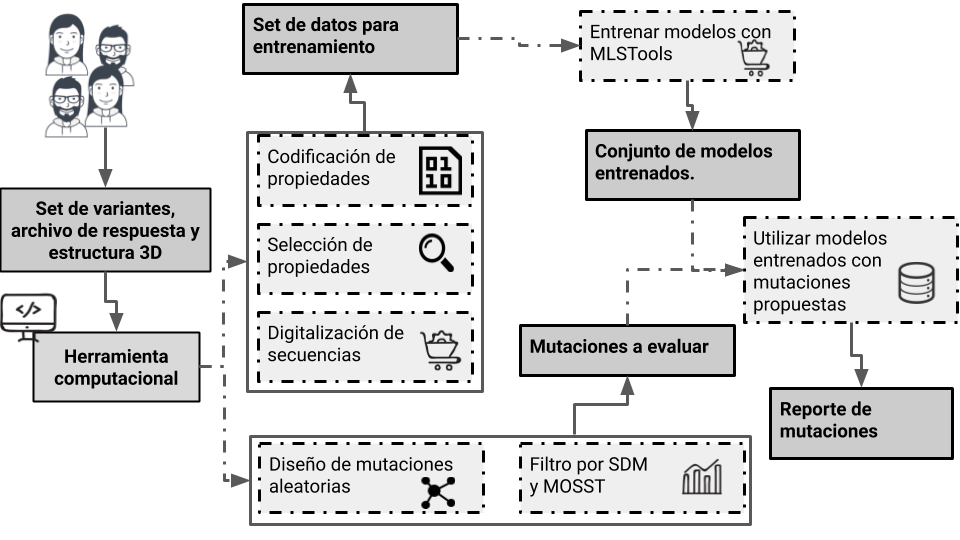
\includegraphics[scale=.4]{fig1.png}
	\caption{Esquema representativo, metodología de digitalización de secuencias.}
	\label{cap3:fig1}
\end{figure}

En una primera instancia, se toma la secuencia y por cada residuo se crea un vector de tamaño $n$ el cual representa el número de propiedades fisicoquímicas descritas en la base de datos AAindex. De esta forma, se crea una matriz de tamaño $r \times n$ donde $r$ representa la cantidad de residuos en la secuencia.


A partir de dicha matriz, técnicas de reducción de dimensionalidad y selección de características son implementadas, utilizando lenguaje de programación Python y la librería scikit-learn \cite{pedregosa2011scikit}, con el fin de seleccionar cuáles son las propiedades más representativas y qué porcentaje de la varianza permiten explicar.

Dado el conjunto de propiedades seleccionadas, se implementarán rutinas basadas en lenguaje de programación Matlab, las cuales reciben el conjunto inicial de datos, en una primera instancia, aplica \textit{zero-padding} con el fin generar vectores de tamaño de potencia de 2, requisito para la aplicación de FFT. A partir de esto, cada columna en el conjunto de elementos, se digitaliza por medio del uso de la transformada rápida de Fourier (FFT) y se obtienen los espectros de frecuencias para cada propiedad fisicoquímica seleccionada previamente.

De esta forma, por cada secuencia, se obtiene un conjunto de espectros de frecuencia, asociados a la digitalización de las propiedades fisicoquímicas seleccionadas mediante técnicas de selección de características.

\subsection{Implementación de modelos de clasificación/regresión para análisis de variantes}

Uno de los objetivos de la codificación de secuencias lineales, es evaluar si el conjunto de espectros de frecuencia para un grupo de variantes, puede ser utilizado como características para generar set de datos y entrenar modelos a partir de estos.

Con esto en mente y apoyados en los conjuntos de datos utilizados para la generación de descriptores basados en propiedades termodinámicas y filogenéticas, expuestos en el capítulo \ref{cap2}, se desarrollarán modelos de clasificación para la evaluación de la estabilidad de proteína y modelos de regresión para la predicción del cambio en la energía libre provocado por los residuos.

En la Figura \ref{cap3:fig3}, se expone un esquema representativo asociado a los pasos a seguir para el desarrollo de los modelos.

\begin{figure}[!h]
	
	\centering
	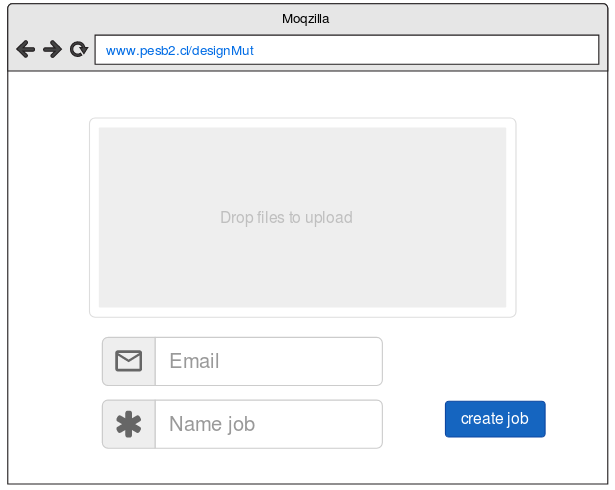
\includegraphics[scale=.4]{fig2.png}
	\caption{Esquema representativo, metodología de clustering se secuencias por medio de espectros de frecuencias basados en propiedades fisicoquímicas.}
	\label{cap3:fig3}
\end{figure}


En una primera instancia, se necesita preparar el conjunto de datos, para ello, se considerarán la secuencia original de la proteína y serán generadas las variantes con respecto a la mutación reportada. De esta forma se creará un conjunto de datos basados en una variante y la respuesta asociada, lo cual corresponde a las diferencias de energía libre que provoca la sustitución del residuo o clasificación de estabilidad.

Al conjunto de secuencias generado, se aplicará la codificación de las propiedades fisicoquímicas, a partir de la información existente en la base de datos AAindex.

Posterior a ello, se seleccionarán las propiedades más informativas y se generará la digitalización de éstas, empleando la metodología descrita en el punto anterior. La selección de las características se basa en un consenso con respecto a las incidencias de cada propiedad en cada secuencia, esto es, dado a que se seleccionan $p$ propiedades por cada secuencia, es posible que diferentes secuencias, presente distintas propiedades. Por lo tanto, se seleccionarán aquellas propiedades que presenten mayor incidencia en el conjunto de secuencias, ya que éstas, serán las más representativas del conjunto completo. 

Una vez se tenga el conjunto de espectros, modelos predictivos serán entrenados aplicando algoritmos de aprendizaje supervisado al set de datos de espectros de frecuencia. Se utilizarán las medidas de desempeño expuestas en el capítulo \ref{cap2}. Los modelos serán validados mediante validación cruzada con un valor de $k=10$, con el fin de evaluar el sobreajuste. 

Finalmente, los resultados a obtener a partir de descriptores basados en espectros de frecuencia, serán comparados con los obtenidos en la fase de exploración de la metodología expuesta en el capítulo 2. Esto con el fin de determinar, qué metodología o caracterización de datos, permite entregar un modelo con mejor desempeño o características deseables. 

Es importante mencionar que, los modelos que se obtengan a partir de la digitalización de propiedades fisicoquímicas, pueden presentar  performance inferior a los modelos a obtener aplicando la metodología del capítulo \ref{cap2}. Sin embargo, si el desempeño es alto, sería suficiente para responder la pregunta planteada. Si son bajos o azarosos, implica que se requiere un mayor refinamiento a la metodología, o, que simplemente el conjunto de datos presenta problemas para entrenar modelos, razón por la cual, debiese descartarse. 

\subsection{Aplicación de técnicas de clustering sobre espectros de frecuencia}

Uno de los supuestos más relevantes asociados al uso de la digitalización y las propiedades fisicoquímicas como descriptores de secuencias lineales, es el hecho de que, proteínas con una misma función, presentan un espectro de frecuencia similar \cite{veljkovic1985possible}. 

Esto, hace pensar que, para un conjunto de secuencias desconocidas, dada una selección de propiedades fisicoquímicas, a la hora de aplicar técnicas de clustering, empleando algoritmos de aprendizaje no supervisado, serán agrupadas de tal forma, que, los espectros de frecuencia en cada grupo presenten similitudes entre ellos, basados en propiedades estadísticas o por medio de análisis cross-espectral.
 
Con el fin de corroborar este supuesto, además de demostrar que el uso de descriptores basados en espectros permite una agrupación de elementos correlacionados con alguna propiedad, en la Figura \ref{cap3:fig2} se expone la metodología planteada.

\begin{figure}[!h]
	
	\centering
	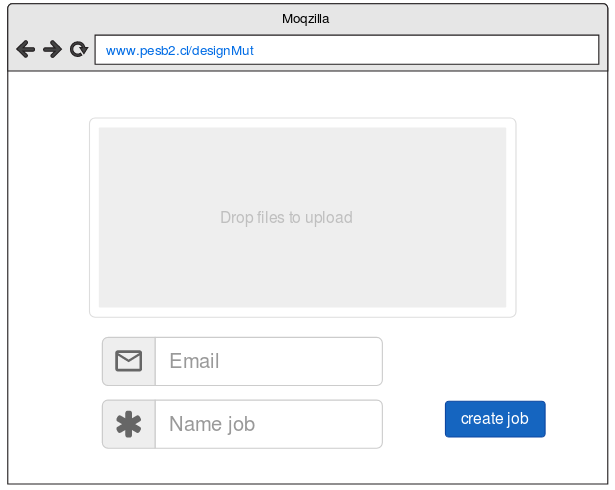
\includegraphics[scale=.4]{fig2.png}
	\caption{Esquema representativo, metodología de clustering se secuencias por medio de espectros de frecuencias basados en propiedades fisicoquímicas.}
	\label{cap3:fig2}
\end{figure}

En una primera instancia, se deberá identificar cuáles son las secuencias de interés, para ello, se trabajarán con diferentes secuencias lineales y variantes asociadas a ellas, principalmente de enzimas, con alguna propiedad característica, proteínas comunes de interés con mutaciones reportadas, etc. La descarga de éstas, se realizará desde diferentes bases de datos, en particular desde Brenda \cite{schomburg2004brenda}, para el caso de las enzimas, Protherm \cite{bava2004protherm} para otras propiedades de interés, relacionadas a estabilidad. 

Es importante mencionar, que no se quiere asociar o reconocer qué efecto causa la mutación. Si no, probar que, proteínas con similar función, tendrán un espectro de frecuencia con características comunes. Es por ello, que la propiedad se conoce de antemano. Sin embargo, también se evaluará si es posible la generación de grupos donde la mutación afecte negativa y positivamente a la estabilidad en proteínas, utilizando para esto, el conjunto de set de datos expuestos en el capítulo \ref{cap2}.

Una vez se tengan las secuencias, se aplicará la codificación de diferentes propiedades fisicoquímicas y a su vez, se digitalizará cada una de éstas. Es importante mencionar, que no se seleccionarán propiedades específicas ya que, puede que las más representativas o informativas no necesariamente generen conjuntos de datos agrupados con el mismo patrón de espectro de frecuencia. 

Esto implica, que se generarán $n$ espectros de frecuencia por cada secuencia y para cada propiedad se aplicarán técnicas de clustering, esto con el fin de determinar si aparecen grupos con misma propiedad conocida, correspondientes a las $n$ propiedades descritas en AAindex. Lo anterior, permitirá evaluar si proteínas con misma funcionalidad, o mismo plegamiento, o, alguna característica en común, quedan agrupadas.

Finalmente, una vez se tengan estos grupos, se realizará la etapa de análisis, caracterización e identificación de patrones. Esto es, en base a la información conocida que se tiene del conjunto de proteínas, evaluar si los grupos formados presentan algo en común, ya sea, propiedades fisicoquímicas, plegamiento, actividad, funcionalidad, etc. 

Esto permitirá evaluar si los espectros de frecuencia, permiten agrupar secuencias con características o patrones en común y si son informativas para dicho objetivo. Se destaca además, que esto implica una fase exploratoria y es incierto lo que pueda resultar. Si bien se postuló las correlaciones entre espectro y propiedad \cite{veljkovic1985possible}, esto fue hecho hace un tiempo prolongado y sólo se evaluaron proteínas o enzimas con particularidades específicas, de esta forma, se espera poder reafirmar dicha afirmación y poder postular un nuevo método de clustering de propiedades en secuencias y sus variantes.

 